\def\difficulty{3}
\sujet{Stereology and Bertrand's paradox}
\index{Stereology}

\begin{note}This tutorial introduces the problems of  stereological measurements, based on simple probes (points, lines...). In a second part, the Bertrand's paradox is explored in the case of the analysis of the distribution of chord lengths of disks and spheres. This tutorial uses the notation that can be found in \cite{Russ2000} (among others).
\end{note} % fin de la note
\vspace*{-10pt}
\begin{center}
{\includegraphics[height=7cm]{spheres2.png}}
\end{center}\vspace*{-10pt}
%\end{figure}
\section{Classical measurements of stereology}\vspace*{-5pt}
Let start by some definitions. The stereology is based on some measures, that can be seen as samples, called probes. A probe can be a point, a line, a curve, a plane, a surface...
These probes allow us to estimate global geometrical properties through partial measures. Very simple and practical probes are now presented and used. The notation $\langle\cdot\rangle$ denotes an expected count for some normalized value.

\begin{center}
\begin{tabular}{|l|l|l|}
\hline
Probe name & Notation & Definition\\ 
\hline
Point count & $\langle P_P\rangle$ & Fraction of points in phase\\ \hline
Line intercept count & $\langle P_L\rangle$ & Number of intersections per length\\ \hline
Area fraction & $\langle A_A\rangle$ & Fraction of area in intersection\\
\hline
\end{tabular}
\end{center}

\subsection{Probes}
 The measures are performed with the following definitions:
\begin{itemize}
 \item $\langle P_P\rangle$: the count of the points that lie in the phase, normalized by the total number of points.
 \item $\langle P_L\rangle$: the count of the number of intersection of lines and the surface of the phase, normalized by the length of the lines included in the objects (in m$^{-1}$, see Fig.\ref{fig:stereology:enonce:PL}). $L_A$ is the ratio between the perimeter of the phase and the total area.
 \item $\langle A_A\rangle$: in a 3D object, the probes are planes and $\langle A_A\rangle$ is the area of the intersections of the planes and the phase, normalized by the total area of the planes.
\end{itemize}
 
\begin{figure}[htbp]
 \centering\caption{Probes examples: points and lines.}%
 \subfloat[Evaluation of $P_P$: count the number of points that lie in the objects, normalized by the total number of points.]{\includegraphics[width=.45\linewidth]{PP.pdf}}\hfill
 \subfloat[Evaluation of $P_L$: count the number of intersection of some lines with the surface of the phase (object). Then, perform a ratio with the total length of the lines.]{\includegraphics[width=.45\linewidth]{PL.pdf}}%
 \label{fig:stereology:enonce:PL}%
\end{figure}


\begin{qbox}
\begin{itemize}
	\item Generate a 2-D binary image containing a population of disks. 
	\item Estimate its area fraction by using points as probe population ($<P_P>=A_A$).
	\item Estimate its length per area by using lines as probe population ($<P_L>=\frac{2}{\pi}L_A$).
	\item Load the 3-D image and verify the following relation: $<A_A>=V_V$ with $V_V$ being the volume fraction.
	\end{itemize}
\end{qbox}


\section{Random chords of a disk, and Bertrand's paradox}\index{Stereology!Random Chords}

The goal of this exercise is to simulate the distribution of random chord lengths on a disk. In the field of process engineering, optical particle sizers provide chord length distributions of objects that are considered as spheres. These developments are not only theoretical, they have a practical use in laboratories or in industrial reactors.

\subsection{Bertrand's paradox}
From Wikipedia\footnote{https://en.wikipedia.org/wiki/Bertrand\_paradox\_(probability)}, the Bertrand paradox goes as follows: Consider an equilateral triangle inscribed in a circle. Suppose a chord of the circle is chosen at random. What is the probability that the chord is longer than a side of the triangle?

Bertrand provided three different methods in order to evaluate this probability. These gave three different values. 

\begin{rmq}The objective is to evaluate the distribution of the chord lengths for two of these methods. The bertrand's paradox lays on the fact that the question is ill-posed, and the choice ``at random'' must be clarified. The reader will find more details in the different citations.
\end{rmq}


\subsection{Random radius}
The intersection of a random line with a disk of radius $R$ is a segment whose half length $r$ is linked to the distance $x$ between the segment and the center of the disk (Eq. \ref{eq:stereology:enonce:radius} and Fig. \ref{fig:stereology:enonce:disk}). 
\begin{equation}
r=\sqrt{R^2-x^2} \label{eq:stereology:enonce:radius}
\end{equation}

\begin{figure}[H]
\centering\caption{Relation between the radius of the chord and the distance to the center of the disk.}%
%\resizebox{10cm}{!}{%
%\input{disk1.tex}
\includegraphics[width=7cm]{section_diskT.png}%
\label{fig:stereology:enonce:disk}%
\end{figure}

\vspace*{-10pt}

As presented in Fig. \ref{fig:stereology:enonce:disk}, $\theta$ is randomly chosen in $[0;2\pi[$ (uniform law), and $x$ is randomly chosen in $[0;R]$ (uniform law). 

\begin{qbox}Repeat the simulation of $r$ by the so-called random radius method a large number of times ($N=1e7$), and compute the probability density function of the distribution.
\end{qbox}
\begin{rmq}This method is in agreement with the analytical results.
\end{rmq}

\vspace*{-6pt}


\subsection{Random endpoints}\vspace*{-2pt}
In this second case, two random angles $\theta_1$ and $\theta_2$ are randomly chosen (uniform law in $[0;2\pi]$). This defines two points and thus a chord (see Fig \ref{fig:stereology:enonce:disk2}). 

\begin{qbox}
Make the simulation for the ``random endpoints'' and compare it to the analytical values and to the first simulation. Notice that this simulation gives different values (search for the Bertrand paradox for more details).
\end{qbox}

\begin{rmq}This method is NOT in agreement with the analytical results.
\end{rmq}

\vspace*{-10pt}

\begin{figure}[H]
 \centering\caption{Second method for simulating a random chord of the disk.}%
 \includegraphics[width=4.5cm]{section_disk2T.png}%
 \label{fig:stereology:enonce:disk2}%
\end{figure}


\subsection{Analytical values}
The probability to obtain a chord of half length $x$ between $a$ and $b$ is given by Eq. \ref{eq:stereology:enonce:disk} (see \cite{Mazzolo2004}):
\begin{equation}
\mathbb{P}(x\in[a;b])=\int_{a}^{b}\frac{\rho}{R\sqrt{R^2-{\rho}^2}}\textrm{d}\rho \label{eq:stereology:enonce:disk}
\end{equation}

\begin{qbox}By discretizing the interval $[0;R]$, compute the analytical value of the probability density function of the distribution of the radii with the Eq. \ref{eq:stereology:enonce:disk}.
\end{qbox}


\section{Random sections of a sphere and a plane}\index{Stereology!Random Planes}
The two previous strategies can be applied on the sphere. What we are looking for are radii of the intersection of the sphere with a random plane.


\subsection{First simulation: random radius}
To find and random plane $\mathcal{P}$ intersecting a sphere $\mathcal{S}$ of radius $R$, one have to choose a direction $\vec{u}$ (i.e. a point on the sphere), find a point $P$ between the latter and the center $O$ of the sphere, and considere the plane $\mathcal{P}$ that is orthogonal to the direction $\vec{u}$ and passing at this point $P$ (Fig. \ref{fig:stereology:enonce:sphere}). 

\begin{qbox}
Code the following method:

\begin{itemize}
 \item A random point on the sphere is chosen with the following method (see \cite{Marsaglia1972}): let $x$, $y$ and $z$ be 3 Gaussian random variables, the point on the sphere is defined by the normed vector $\vec{u}$, such that:
 
 \begin{equation}
  \vec{u}=\frac{1}{\sqrt{x^2+y^2+z^2}}\colvec{3}{x}{y}{z}\label{eq:stereology:enonce:pointsphere}
 \end{equation}

 \item The point $P$ is chosen as $\vec{OP}=\alpha\vec{u}$, with $O$ being the center of the sphere, and $\alpha$ being a uniform random variable in $[0;R]$. The plane $\mathcal{P}$ is orthogonal to $\vec{u}$, passing at $P$ (see Fig. \ref{fig:stereology:enonce:sphere}).
\end{itemize}
\end{qbox}
Notice that this simulation is equivalent to the first presented case (random radius) of the random chords of a disk, and that the choice of the random point on the sphere is useless.

\begin{figure}[htbp]
 \centering\caption{First simulation method of a random intersection  of a sphere and a plane.}%
 \includegraphics[width=10cm]{section_sphere.png}%
 \label{fig:stereology:enonce:sphere}%
\end{figure}

\begin{rmq}The method that consists to choose a point by two angles does not provide a uniform distribution of the points on the sphere.
\end{rmq}


\subsection{Second simulation: 3 random endpoints}
The random plane $\mathcal{P}$ is defined by 3 random points laying on the sphere (see Eq. \ref{eq:stereology:enonce:pointsphere}). 

\begin{qbox}
\begin{itemize}
 \item Analytically, find the distance between the center of the sphere $O$ and the plane $\mathcal{P}$.
 \item Simulate a high number of intersections and find numerically the distribution of the radii of these intersection disks.
\end{itemize}

\end{qbox}

\subsection{Third simulation: 2 random endpoints}
Choose 2 random points laying on the sphere (see Eq. \ref{eq:stereology:enonce:pointsphere}) and evaluate their half distance.

\begin{qbox}
Simulate a high number of couple of points and evaluate the distribution of their half distances.
\end{qbox}

\begin{rmq}The distribution of the length of the chords on a sphere is linear, and is different from the distribution of the radii resulting from the intersection of a random plane and the sphere.
\end{rmq}


\subsection{Comparison}
\begin{qbox}Compare the 3 results and comment.
 
\end{qbox}


% \section{Sections of a population of spheres}
% \begin{qbox}
% \begin{itemize}
% %\item First, establish analytically the distance $\parallel\vec{OP}\parallel$ between a point $O$ and the nearest point $P$ on the plane $\mathcal{P}$, as a function of $A$ a point of $\mathcal{P}$, and $\vec{n}$ the vector normal to $\mathcal{P}$.
% 
% \item Simulate the population of $N$ spheres, so that these spheres do not intersect. I might be useful to use a Delaunay triangulation of the centers of the spheres in order to get the maximal radius that can be used.
% 
% \item Construct a random plane by the choice of 3 point on the sphere that surrounds the simulation space.
% 
% \item Last, compute the radii of the intersections of the plane and the spheres. Repeat this step a large amount of times, so that a distribution of the radii can be constructed. Verify that this simulation agrees the previous analytical result.
% \end{itemize}
% \end{qbox}
% 
% When dealing with a population of different sizes of spheres, a particular size of intercept disk could result from the intersection of the plane with several different sphere sizes. The resulting 2-D radii distribution would show the superposition of data from the different 3-D spheres in proportion to their
% relative abundance and to their size. The 3-D radii distribution might be unfolded sequentially.
% For the case of spheres, this method was first described by \cite{Saltikov1967} and has been subsequently refined by many others, such as \cite{Cruz-Orive1976}. The method is simply to solve a set of simultaneous equations in which the independent variables are the number $N_A$ of disks of various sizes (measured on the images and recorded as a histogram) using a coefficient matrix $K$, to obtain the numbers of spheres $N_V$ of each size present in the material:
% \begin{equation}
% N_A=2R_{max}K.N_V \label{eq:stereology:enonce:populationspheres}
% \end{equation}
% where $R_{max}$ is the maximal radius of disks/spheres.
% 
% The matrix $K$ is determined by calculating, from geometric probability, the frequency distribution for the number of disks in each size class due to three dimensional objects of each size. For spheres, $K$ can be solved analytically (see the previous exercise):
% \begin{equation}
% K_{i,j}=\left\{\begin{array}{cc}
% \displaystyle\frac{1}{n}\left(\sqrt{j^2-(i-1)^2}-\sqrt{j^2-i^2}\right)& \textrm{for } j\geq i\\
% 0 & \textrm{otherwise}
% \end{array}\right.
% \end{equation}
% where $n$ is the number of histogram bins.
% 
% By inverting Eq. \ref{eq:stereology:enonce:populationspheres}, it is possible to retrieve the 3-D size distribution of spheres:
% \begin{equation}
% N_V=\frac{1}{2R_{max}}K^{-1}.N_A
% \end{equation}
% 
% 
% \begin{qbox}
% \begin{itemize}
% 	\item Load the 3-D binary image and the disk radii used for generating the spheres.
% 	\item Calculate the radii of the disks coming from different sections of the 3-D image. Deduce the distribution of disk radii $N_A$.
% 	\item Calculate the matrix $K$.
% 	\item Estimate the distribution of sphere radii $N_V$.
% 	\item Compare this estimation with the real distribution.
% \end{itemize}
% \end{qbox}
